Here goes an introduction to this chapter and the sections to come.


\section{Requirements}

Being a project that is experimental and research-oriented in style, the
requirements could not be rigidly determined in fine detail at the outset, or
even at later stages. However it was certainly possible, and indeed important,
to establish a set of high-level requirements and guiding principles for the
project. These were categorised as functional and non-functional requirements.

\subsection{Functional Requirements}

\begin{itemize}
\item The program must take a Scheme program as input and output a Lua program
as output
\item When the Lua output from the program is run through a Lua interpreter, it
must produce the same output as the Scheme program run natively through a Scheme
interpreter.
\end{itemize}

The point about the eventual program output raises an interesting question;
should the output ultimately look like Scheme data or its equivalent Lua data?
The answer to this involves another question around the program's use. In a role
as a kind of Scheme interpreter, the automatic choice would be to use Scheme
data, but perhaps a translator in the true sense should output only Lua data.
It was decided that the output should exactly match the Scheme output, mainly
because this allowed direct comparison of output with a native Scheme
interpreter, which simplified testing. As will be seen later, it turns out that
changing the format of the output to look like Lua is a trivial matter in any
case.

\subsection{Non-functional Requirements}

\begin{itemize}
\item The running time of the resulting Lua program should be as short as
possible
\item The output of the program should be readable Lua code as much as possible
\end{itemize}

In particular, the non-functional requirements, though in conflict with each
other to a certain extent, pointed to simplicity as a primary design objective.


\section{Design And Implementation}


\subsection{First Approach}

The initial approach involved finding for each construct in Scheme, its most
precise and efficient representation in Lua. In French parlance, this is nicely
described by the phrase ``le mot juste'', meaning ``the precise word'' or ``the
perfect word'', and it brings to mind the image of an expert translator of
human languages, who knows through experience how to accurately convey the
intended semantic of each phrase from one language to another for a particular
context.  At first, this seemed like a reasonable and credible way of
proceeding given the small size of the core of the Scheme language.

However it soon became apparent that this approach would quickly become
unwieldy, as the range of various contexts in which an expression could appear
often meant the optimal translation needed to be adjusted slightly. An example
of this is\ldots

\subsection{Second Approach}

\begin{figure}
\centering
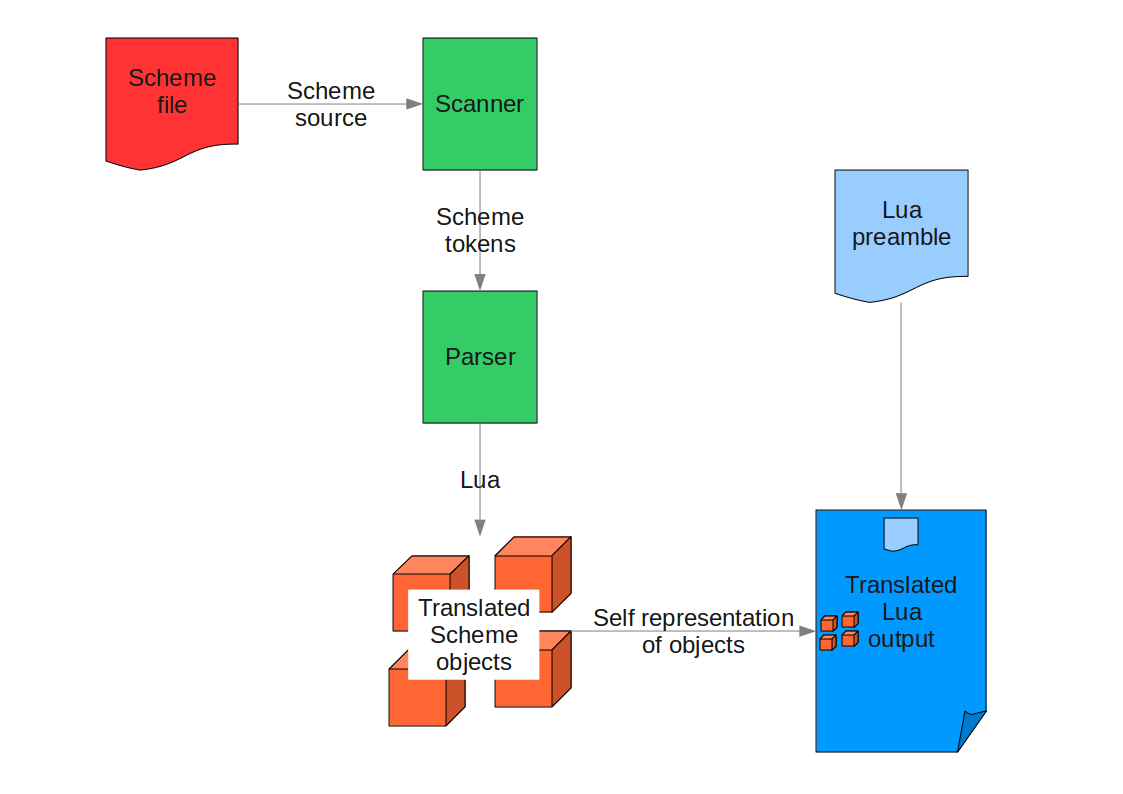
\includegraphics[width=\textwidth]{overview.png}
\caption{Overall structure of the translator}
\label{fig:overview}
\end{figure}

This approach was more structured in its implementation.


\section{Features}

\subsection{Data Types}

\begin{itemize}
\item Atomic Data: Booleans, Numbers, Characters and Strings.
\item Compound Data: Lists, Vectors and Bytevectors
\end{itemize}

We will look at each of these in turn to identify what commonalities or
differences between Scheme and Lua could affect the translation.

\subsubsection{Booleans}

Being a very simple data type and having only two possible values, booleans are
easily translated. In Lua, the values are \texttt{true} and \texttt{false},
corresponding to \texttt{\#t} and \texttt{\#f} respectively in Scheme.

\subsubsection{Numbers}

Scheme has a very rich syntax for describing numbers. This is in contrast with
Lua, in which the double precision floating point number is the only
numeric type~\cite[p.10]{luabook}.

\subsubsection{Strings}

Scheme strings are more restrictive than Lua strings. ''Lua is
eight-bit clean and its strings may contain characters with any numeric code,
including embedded zeros. This means that you can store any binary data into a
string''~\cite[p.11]{luabook}.

\subsubsection{Lists}

Lists are the primary data type in Scheme, and there is a duality in the
representation of list data and the core syntax of a Scheme program.

\subsubsection{Vectors and Bytevectors}

Vectors are similar to lists.

\subsection{Branching}

Scheme has a number of constructs for branching.

\subsection{Looping}

Including tail recursion

\subsection{Continuations}

One shot continuations using coroutines

\subsection{Syntax Extension}

syntax-rules etc.


\section{Components}

\subsection{Main Program}

The entry point to the translator consists of a shell script that calls the main
\texttt{scheme2lua.lua} program, which contains the main loop. It take a number
of scheme input files as arguments and writes the lua translation to standard
output. The usage is outlined below:

\begin{framed}
\texttt{\$ ./scheme2lua [input-file] \ldots}
\end{framed}

The \texttt{scheme2lua.lua} program is a filter, which takes scheme from its
standard input and outputs lua to standard output. It does this through a loop
that repeatedly calls the \texttt{parse} function on the next token of input,
until none remains. Below is the algorithm for the main loop:

\begin{framed}
Algorithm for main loop
\end{framed}

\subsection{The Scanner}

\begin{figure}
\centering
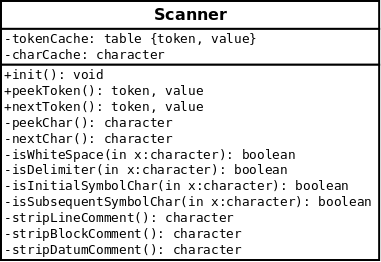
\includegraphics[width=\textwidth]{scannerUML.png}
\caption{A UML class diagram of the scanner component}
\label{fig:scannerUML}
\end{figure}

The scanner component is used to read the input file(s) and split them into a
stream of atomic tokens, which are supplied to the parser. Scanners are a common
component in compilers and interpreters and, rather than attempt to ``re-invent
the wheel'', a standard approach to scanning was followed for this project.
Though it used a slightly different implementation, it was created borrowing
heavily from the ideas and techniques used in the SAL interpreter\cite{sal}.

Figure~\ref{fig:scannerUML} shows the structure of the scanner in UML class
form. As can be seen from the diagram, the scanner is accessible through three
methods: \texttt{init()} initialises the scanner; the others both return
individual tokens from the scanner---the difference being that
\texttt{peekToken()} leaves the returned token in the scanner, whereas
\texttt{nextToken()} does not. Internally, there are helper functions for
dealing with caching, comments and recognising the various Scheme tokens.

\subsection{The Parser}

\begin{figure}
\centering
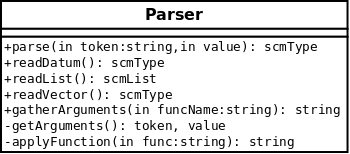
\includegraphics[width=\textwidth]{parserUML.png}
\caption{A UML class diagram of the parser component}
\label{fig:parserUML}
\end{figure}

See figure~\ref{fig:parserUML} for a diagrammatic representation of the parser
component.

\subsection{Intermediate Data Types}

\begin{figure}
\centering
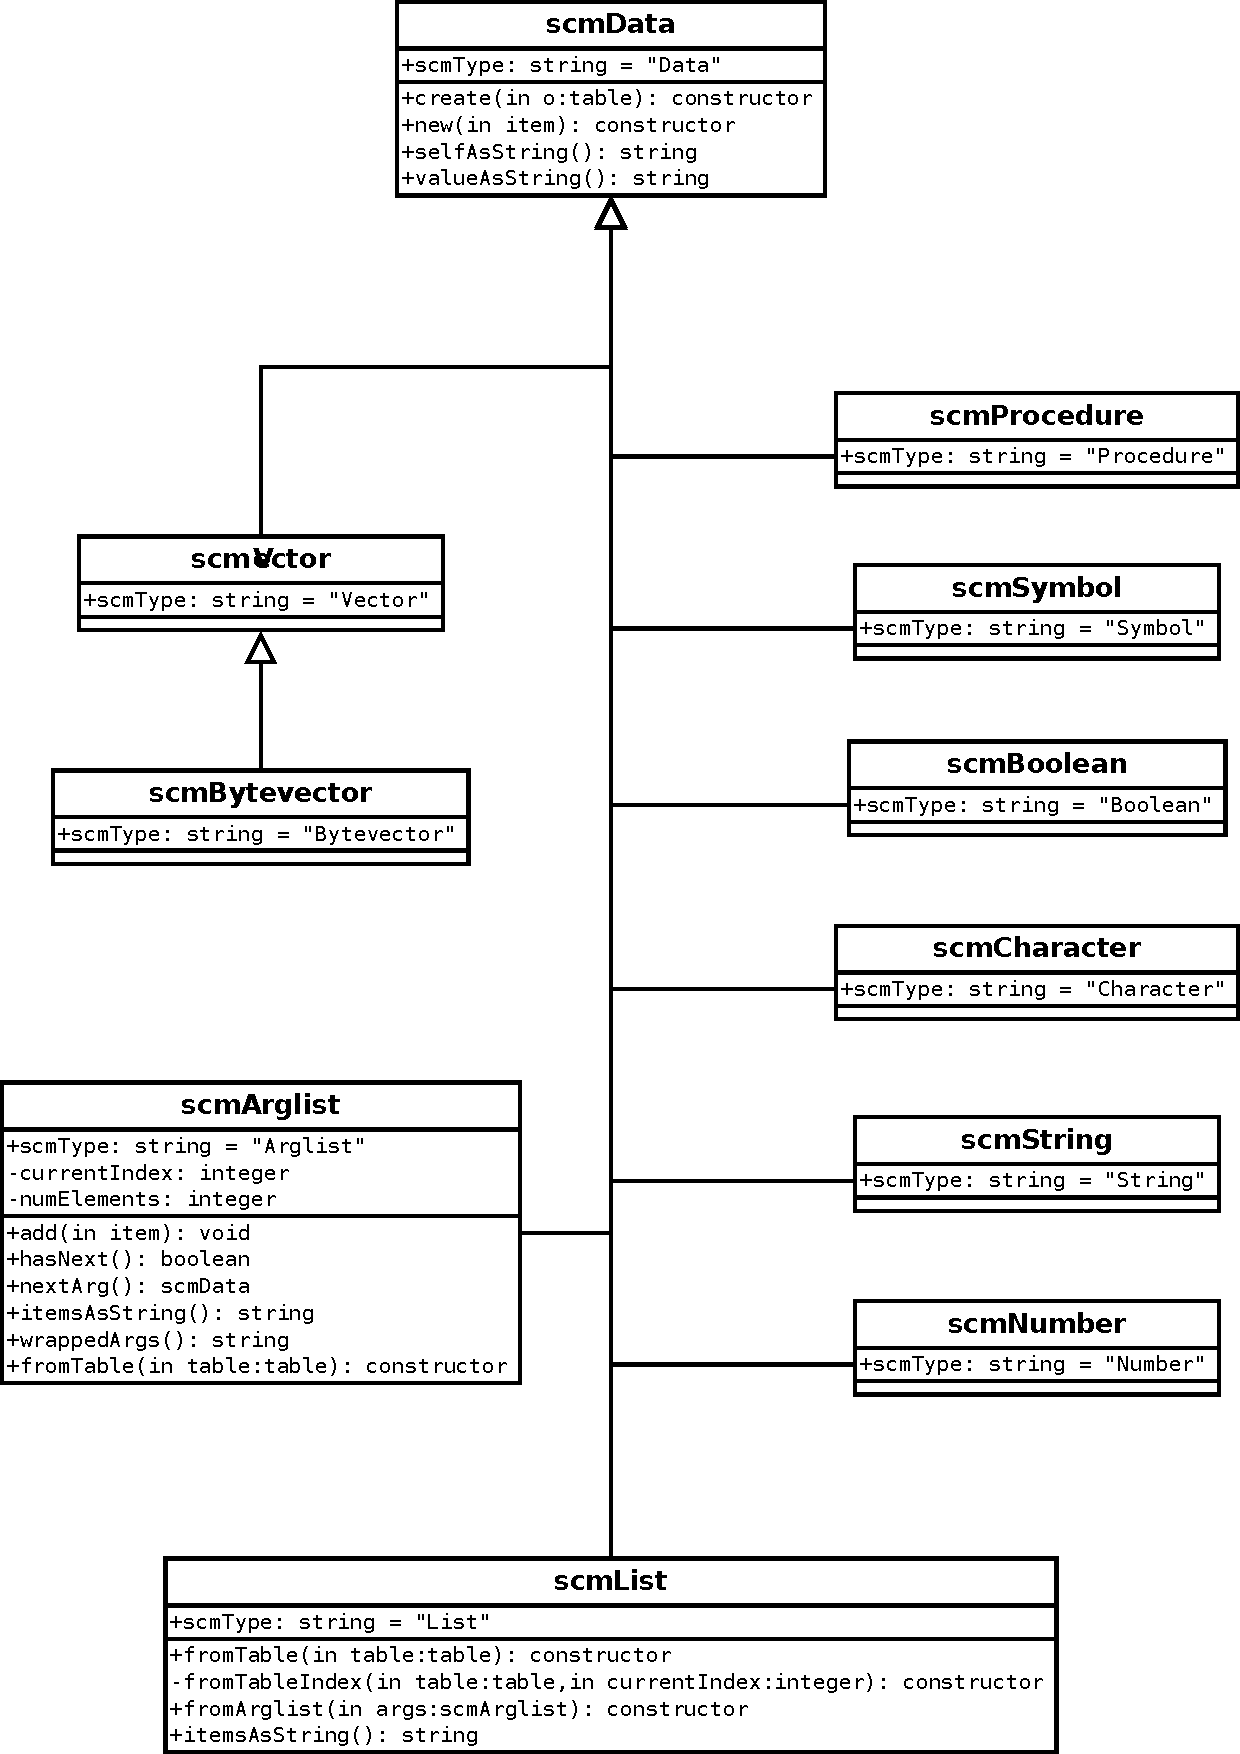
\includegraphics[width=\textwidth]{scmDataUML.pdf}
\caption{The structure of the intermediate data types}
\label{fig:scmDataUML}
\end{figure}

As can be seen in figure~\ref{fig:scmDataUML}


\section{The Operation Of A Translated Program}

The output of the translator consists of two main parts:
\begin{itemize}
\item A library of supported Scheme functions and operations, written in Lua.
This is identical for every translation.
\item The translated output of the the scheme input program, which uses a subset
of the library to carry out its purpose.
\end{itemize}

All of the functions of the library deal with data in the intermediate form, as
output by the parser. That is to say that all function arguments and all of the
return values are in this form.
